\documentclass[a4paper, oneside, final]{scrartcl} 
\usepackage[margin=1in]{geometry}
\usepackage{titlesec} % Allows creating custom \section's
\usepackage{graphicx}
\usepackage{lipsum}
\usepackage{scrpage2} % Provides headers and footers configuration
\usepackage{marvosym} % Allows the use of symbols
\usepackage{tabularx,colortbl} % Advanced table configurations
\usepackage{hyperref}
\usepackage{booktabs}
\usepackage{ltablex}
\usepackage[utf8]{inputenc}

\titleformat{\section}{\Large\scshape\raggedright}{}{0em}{}[\titlerule] % Section formatting

\pagestyle{scrheadings} % Print the headers and footers on all pages

\addtolength{\voffset}{-0.5in} % Adjust the vertical offset - less whitespace at the top of the page
\addtolength{\textheight}{3cm} % Adjust the text height - less whitespace at the bottom of the page

\newcommand{\gray}{\rowcolor[gray]{.90}} % Custom highlighting for the work experience and education sections
\newcommand\YUGE{\fontsize{30}{60}\selectfont}

\begin{document}

\pagenumbering{gobble}% Remove page numbers (and reset to 1)

%\begin{flushleft}
\begin{center}
\YUGE \textsc{Diego Bruciaferri}\\
\end{center}
\bigskip%\bigskip
\textsc{University of Plymouth}, \hspace{3.9cm} \textsc{E-mail}: \href{mailto:diego.bruciaferri@plymouth.ac.uk}{diego.bruciaferri@plymouth.ac.uk}\\
\textit{Faculty of Science and Engineering}, \hspace{5.2cm} \textsc{mobile}: +44 7490 444 958\\
Marine building, $3^{rd}$ floor, \hspace{7.85cm} \textsc{Citizenship}: Italian\\
Drake Circus, Plymouth, \hspace{5.4cm} \url{http://www.coastalprocesses.org/}\\
Devon, PL4 8AA,\\
United Kingdom \\
%\end{flushleft}
%\begin{center}
%\noindent\rule{6cm}{1.8pt}\\
%\end{center}
%\vspace{0.cm}
%-----------------------------------------------------------------------------------------------------

\section{Research interests}
\normalsize
\noindent
My research in geophysical and environmental fluid dynamics mainly focusses on the turbulent ocean dynamics arising from the interplay between the atmosphere and the ocean surface and it involves the usage of numerical models and observations.   Of particular interest to me is the role of the mesoscale dynamics in controlling the ocean hydrodynamics and how to improve its representation in numerical ocean models. During my MSc and research assistant positions I worked on the coupling of Eulerian ocean and waves numerical models as well as the development and improvement of Lagrangian passive and active tracer models. My current Ph.D. research involves the numerical modelling of shelf seas. My goal is to improve the capability of current Ocean General Circulation models to adequately simulate the shelf seas dynamics. During my PhD research I developed a new vertical coordinate system for numerical ocean modelling and I applied it to study the hydrodynamics of the Black Sea and the Dead Sea.
%-------------------------------------------------------------------------------------------------------

\section{Education}
\normalsize
\noindent

\label{tab:daypack}
\begin{tabularx}{\linewidth}{>{\raggedright\scshape}p{4.4cm}|X}
\gray Degree:       & \textbf{Ph.D. in Physical Oceanography}\\
\gray Period:       & \textbf{2015 --- 2019}\\[6pt]
\gray University:   & \textsc{University of Plymouth}, Plymouth, United Kingdom\\
\gray Thesis Title: & \textit{Advanced methods for numerical modelling of regional seas}\\[3pt]
\gray Supervisors:  & \textbf{1st}: Prof. Georgy Shapiro (DoS, University of Plymouth)\\
\gray              & \textbf{2nd}: Prof. Tal Ezer (Old Dominion University)\\
\gray              & \textbf{3rd}: Dr.   Fred Wobus (University of Plymouth)\\
\end{tabularx}

%\medskip

\begin{tabularx}{0.97\linewidth}{>{\raggedright\scshape}p{4.4cm}|X}
\gray Degree:       & \textbf{M.Sc. in Environmental Sciences} \\
\gray Period:       & \textbf{2011 --- 2014}\\
\gray Rank:         & $110/110$, with distinction (\textit{magna cum laude})\\
\gray University:   & \textsc{University of Bologna}, Bologna, Italy\\
\gray Thesis Title: & \textit{Study of a wind-wave numerical model and its integration with an ocean and an oil-spill numerical models}\\[3pt]
\gray Supervisors:  & \textbf{1st}: Prof. Nadia Pinardi (DoS, University of Bologna)\\
\gray              & \textbf{2nd}: Dr. Michela De Dominicis (Instituto Nazionale di Geofisica e Vulcanologia)\\
\end{tabularx}

%\medskip

\begin{tabularx}{0.97\linewidth}{>{\raggedright\scshape}p{4.4cm}|X}
\gray Degree:       & \textbf{B.Sc. in Marine Biology and Physical Oceanography} \\
\gray Period:       & \textbf{2007 --- 2011}\\
\gray Rank:         & $100/110$ \\
\gray University:   & \textsc{Politecnico delle Marche}, Ancona, Italy\\
\gray Thesis Title: & \textit{Implementation of an ocean numerical model to study the dispersion dynamics, in the marine environment, of a cooled and chlorinated seawater discharge coming from a LNG-FSRU terminal}\\[3pt]
\gray Supervisors  & \textbf{1st}: Dr. Aniello Russo (DoS, Politecnico delle Marche)\\
\end{tabularx}

%-------------------------------------------------------------------------------------------------------

\section{Professional Experience}
\noindent
\normalsize
\begin{tabularx}{0.97\linewidth}{>{\raggedright\scshape}p{4.4cm}|X}
\gray \textsc{Research Title:} & \textbf{Shelf Seas Scientist}\\
\gray \textsc{Period:}         & \textbf{Aug 2019 - present}\\
\textsc{Employer:}             & \textsc{UK Met Office}  \\
                               & \textsc{Ocean Forecasting Research {\&} Development Group}, Exeter, United Kingdom \\
                               & \\
\textsc{Main activities}       & \textbf{Ocean Modelling - R{\&}D} \\
\textsc{and responsibilities:} & \\
\end{tabularx}

\begin{tabularx}{0.97\linewidth}{>{\raggedright\scshape}p{4.4cm}|X}
\gray \textsc{Research Title:} & \textbf{Post-Doctoral Researcher}\\
\gray \textsc{Period:}         & \textbf{Jun 2019 - Jul 2019}\\
\textsc{Employer:}             & \textsc{University of Plymouth}  \\
                               & \textsc{Plymouth Ocean Forecasting Centre}, Plymouth, United Kingdom \\
                               & \\
\textsc{Main activities}       & \textbf{Ocean Modelling - R{\&}D} \\
\textsc{and responsibilities:} & \\
\end{tabularx}

\begin{tabularx}{0.97\linewidth}{>{\raggedright\scshape}p{4.4cm}|X}
\gray \textsc{Research Title:} & \textbf{Ph.D. Researcher}\\
\gray \textsc{Period:}         & \textbf{Oct 2015 - May 2019}\\
\textsc{Employer:}             & \textsc{University of Plymouth}  \\
                               & \textsc{Coastal Processes Research Group} and \\
                               & \textsc{Plymouth Ocean Forecasting Centre}, Plymouth, United Kingdom \\
                               & \\
\textsc{Main activities}       & $\bullet$ \textbf{Scientific responsible} of \textbf{EMODnet - Black Sea} \\
\textsc{and responsibilities:} & \textbf{Checkpoint} challenge Coast \url{http://emodnet-blacksea.eu/}) (challenge leader is Prof. Georgy Shapiro, University of Plymouth). \\
                               & $\bullet$ \textbf{Teaching assistant} for \\
                               & \ \ $\ast$ \textsc{Shelf Seas and Estuaries} (B.Sc.)\\
                               & \ \ \ \ (\textit{Module Leader: Prof. G.I.Shapiro})\\
                               & \ \ $\ast$ \textsc{Introduction to Ocean Modelling} (B.Sc.)\\
                               & \ \ \ \ (\textit{Module Leader: Prof. G.I. Shapiro})\\
                               & \ \ $\ast$ \textsc{Modelling Marine Processes} (M.Sc.)\\
                               & \ \ \ \ (\textit{Module teacher: Prof. G. I. Shapiro})\\
\end{tabularx}

%\medskip

\begin{tabularx}{0.97\linewidth}{>{\raggedright\scshape}p{4.4cm}|X}
\gray \textsc{Research Title:}  & \textbf{Senior Ocean Modeller}\\
\gray \textsc{Period:}          & \textbf{Sep 2017 - Mar 2018}\\
\textsc{Employer:}        & \textsc{University of Plymouth} \\
                          & \textsc{Plymouth Ocean Forecasting Centre}, Plymouth, United Kingdom\\
                                & \\
\textsc{Main activities}        & $\bullet$  \textbf{Ocean Modeller} for \textbf{Institutional Links STREAM} \\
\textsc{and responsibilities:}  & \textbf{2016 Grant} - \textit{Physical mechanisms which control water budget and sea level in the Dead Sea}. Partners of the project are \\
                                 & \ \ $\ast$ \textsc{University of Plymouth} (Prof. Georgy Shapiro \\
                                 & \ \ \ \ \ is P.I.) \\ 
                                 & \ \ $\ast$ \textsc{University of Jordan} (Prof. Riyad Manasrah) \\
                                 & \ \ $\ast$ \textsc{Israel Oceanographic and Limnological} \\
                                 & \ \ \ \ \ \textsc{Research National Institute} (Dr. Isaac Gertman). \\
                                 & The aim of the project is to test the hypothesis that the observed step-like structures in the Dead Sea have a significant effect on the rate of evaporation and hence the drop of the sea level. A numerical study is performed and the NEMO ocean model is modified and adapted to simulate the Dead Sea hydrodynamics. \\
\end{tabularx}
%\pagebreak
%\medskip


\begin{tabularx}{0.97\linewidth}{>{\raggedright\scshape}p{4.4cm}|X}
\gray \textsc{Research Title:}  & \textbf{Research Assistant}\\
\gray \textsc{Period:}          & \textbf{2014 - 2015}\\
\textsc{Employer:}        & \textsc{Istituto Nazionale di Geofisica Vulcanologia - INGV} \\
                          & \textit{National Institute of Geophysics and Volcanology},\\
                          & \textit{National Group of Operational Oceanography} GNOO\\         
                           & Bologna, Italy\\
                                 & \\
\textsc{Main activities}        & $\bullet$ Member of the \textbf{NEMO} Ocean General Circulation Model \\
\textsc{and responsibilities:}  & \ \ \textbf{System Team} (\textbf{NEMO WAVE WORKING group}) \\
                                & $\bullet$ \textbf{Research and development} of the \textbf{MEDSLIK-II oil spill model} (open source model, \url{http://medslikii.bo.ingv.it/}) \\                                  
                                & $\bullet$ \textbf{Development} of the web infrastructure for the integration of MEDSLIK-II in the \textbf{MEDESS 4MS} european project (Mediterranean Decision Support System for Marine Safety, \url{http://www.medess4ms.eu/}) \\
                                & $\bullet$ \textbf{Researcher on board} of \textbf{MEDESS4MS oceanographic cruises} (Serious Games) at Palma de Mallorca and Elba islands: numerical models and multi-platform observations (satellite, drifters) have been used to evaluate the forecast skills of the MEDESS4MS system during oil pollution episodes.\\
                                & $\bullet$  \textbf{Oil spill modeller} for \textbf{EMODnet - MedSea Checkpoint} - Human Activities sub-portal \url{http://www.emodnet-mediterranean.eu/})\\
                                & $\bullet$ \textbf{Research and development} of the \textbf{SURF} (Structured Unstructured Relocatable model for Forecasting) wind-wave module in collaboration with the SiNCEM (Laboratorio di Simulazioni Numeriche del Clima e degli Ecosistemi Marini - Laboratory of Numerical Simulations of Climate and Marine Ecosystems) research group of the Alma Mater Studiorum University of Bologna within the TESSA project. \\
\end{tabularx}          

\newpage

%-------------------------------------------------------------------------------------------------------
\section{Publications}
\noindent
\normalsize

\begin{itemize}
\item \textbf{Bruciaferri, D.}, Shapiro, G., Stanichny, S., Zatsepin, A., Ezer, T., Wobus, F., Francis, X., Hilton, D. \textit{The development of a 3D computational mesh to improve the representation of dynamic processes: the Black Sea test case} (\textit{submitted to Ocean Modelling}).
%\item Shapiro, G.,Gertman, I., Manasrahc, R.,  \textbf{Bruciaferri, D.}. \textit{The effect of thermohaline staircases on the sea level in the Dead Sea}.(\textit{submitted to Journal of Marine Systems}).
\item \textbf{Bruciaferri, D.}, Shapiro, G.I. and Wobus, F. (2018) \textit{A multi-envelope vertical coordinate system for numerical ocean modelling}. Ocean Dynamics, Volume 68(10), Pages 1239-1258, \url{https://link.springer.com/article/10.1007\%2Fs10236-018-1189-x}. 
\item M. De Dominicis, \textbf{D. Bruciaferri}, R. Gerin, N. Pinardi, P.M. Poulain, P. Garreau, G. Zodiatis, L. Perivoliotis, L. Fazioli, R. Sorgente, C. Manganiello, \textit{A multi-model assessment of the impact of currents, waves and wind in modelling surface drifters and oil spill}, Deep Sea Research Part II: Topical Studies in Oceanography, Volume 133, November 2016, Pages 21-38, ISSN 0967-0645, \url{http://dx.doi.org/10.1016/j.dsr2.2016.04.002}.\\
\item F. Trotta, E. Fenu, N. Pinardi, \textbf{D. Bruciaferri}, L. Giacomelli, I. Federico, G. Coppini, \textit{A Structured and Unstructured grid Relocatable ocean platform for Forecasting (SURF)}, Deep Sea Research Part II: Topical Studies in Oceanography, Volume 133, November 2016, Pages 54-75, ISSN 0967-0645, \url{http://dx.doi.org/10.1016/j.dsr2.2016.05.004}.
%\pagebreak
\item G. Zodiatis, M. De Dominicis, L. Perivoliotis, H. Radhakrishnan, E. Georgoudis, M. Sotillo, R.W. Lardner, G. Krokos, \textbf{D. Bruciaferri}, E. Clementi, A. Guarnieri, A. Ribotti, A. Drago, E. Bourma, E. Padorno, P. Daniel, G. Gonzalez, C. Chazot, V. Gouriou, X. Kremer, S. Sofianos, J. Tintore, P. Garreau, N. Pinardi, G. Coppini, R. Lecci, A. Pisano, R. Sorgente, L. Fazioli, D. Soloviev, S. Stylianou, A. Nikolaidis, X. Panayidou, A. Karaolia, A. Gauci, A. Marcati, L. Caiazzo, M. Mancini, \textit{The Mediterranean Decision Support System for Marine Safety dedicated to oil slicks predictions}, Deep Sea Research Part II: Topical Studies in Oceanography, Volume 133, November 2016, Pages 4-20, ISSN 0967-0645, \url{http://dx.doi.org/10.1016/j.dsr2.2016.07.014}.
\end{itemize}
%\pagebreak
%-------------------------------------------------------------------------------------------------------
\section{Conferences}
\noindent
\normalsize
\begin{itemize}

\item \textbf{D. Bruciaferri}, G. Shapiro, S. Stanichny, A. Zatsepin, T. Ezer, F. Wobus, X. Francis and D. Hilton. \textit{A new numerical model for the Black Sea circulation}. Geophysical Research Abstracts. Vol. 21, EGU2019-5933, 2019, April 2019 (\textit{Oral}).
\item \textbf{D. Bruciaferri}, G. Shapiro, S. Stanichny, A. Zatsepin, T. Ezer, F. Wobus, X. Francis and D. Hilton. \textit{A numerical model of the Black Sea circulation using a structured multi-envelope mesh with variable resolution}. Met Office seminars, $5^{th}$ March 2019, Exeter (UK) (\textit{Oral}).
\item \textbf{D. Bruciaferri}, G. Shapiro, S. Stanichny, A. Zatsepin, T. Ezer, F. Wobus, X. Francis and D. Hilton. \textit{An advanced numerical model of the Black Sea}. PlyMSEF conference, Plymouth Marine Laboratoty, $5^{th}$ February 2019, Plymouth (UK) (\textit{Oral}).
\item G. I. Shapiro, R. Manasrah, I. Gertman and \textbf{D. Bruciaferri}. \textit{The effect of different types of water column structure on the sea level in the Dead Sea}. Geophysical Research Abstracts. Vol. 20, EGU2018-19780, April 2018 (\textit{Poster}).
\item \textbf{D. Bruciaferri}, G. I. Shapiro and F. Wobus. \textit{An Advanced Vertical Coordinate System to Improve the Representation of the Oceanic Transport in Regional Non-Isopycnal Ocean Models}. Abstract 310863 presented at 2018 Ocean Sciences Meeting, Portland, OR, 12-16 February 2018 (\textit{Oral}).
\item \textbf{D. Bruciaferri}, G. I. Shapiro and F. Wobus, \textit{The development of an advanced vertical discretisation scheme for a regional ocean model}. Geophysical Research Abstracts. Vol. 19, EGU2017-7276, April 2017 (\textit{Poster}).
\item \textbf{D. Bruciaferri}, G. I. Shapiro, F. Wobus, \textit{A coupled ocean-wave modeling system to investigate the role of the wave-induced turbulence on the Cold Intermediate Water formation in the Black Sea - The scientific approach}, NPOP conference, Bristol (UK), April 2016 (\textit{Poster}).
\item M. De Dominicis, N. Pinardi, \textbf{D. Bruciaferri}, S. Liubartseva, \textit{Numerical modelling for real-time forecasting of marine oil pollution and hazard assessment}, EGU assembly 2015.
\end{itemize}
%\pagebreak
%-------------------------------------------------------------------------------------------------------
\section{Technical Reports}
\noindent
\normalsize
\begin{itemize}
\item B. B. Romain, P. A. Bouttier, C. Bricaud, \textbf{D. Bruciaferri}, J. Chanut, S. A. Ciliberti, E. Clementi, A. Coward, D. Delrosso, C. Ethé, S. Flavoni, T. Graham, J. Harle, D. Iovino, D. Lea, C. Lévy, T. Lovato, G. Madec, N. Martin, S. Masson, P. Mathiot, S. Mocavero, G. Nurser, E. O’Dea, J. Paul, C. Rousset, D. Storkey, A. Storto, 2016, \textit{Main achievements for NEMO evolution during MyOcean period}, Mercator Ocean Journal, 54
\item \textbf{D. Bruciaferri} and the MEDSLIK-II System Team, 2016. MEDSLIK-II, \textit{Lagrangian marine surface oil spill model, User Manual, Version 1.02}. \url{http://medslikii.bo.ingv.it/}.\\
\end{itemize}
%-------------------------------------------------------------------------------------------------------
\section{Grant}
\noindent
\normalsize
\begin{itemize}
\item  \textbf{BSc thesis bursary} offered by Ancona district \hspace{3.cm} \textbf{02/2010 - 11/2011} \\
         and ECOTECH SYSTEMS (ETS srl)\\
\item  \textbf{PlyMSEF Grant-In-Aid} offered by Plymouth Marine Science \hspace{2.4cm} \textbf{02/2019} \\
         and Education Foundation (PlyMSEF)\\      
\end{itemize}
%-------------------------------------------------------------------------------------------------------
\pagebreak
\section{Specialised Education}
\noindent
\normalsize

\begin{tabularx}{0.97\linewidth}{>{\raggedright\scshape}p{4.4cm}|X}
\gray PG Course: & \textbf{Fluid Dynamics Summer School}\\
\gray Period:    & \textbf{September 2016}\\
Institute:       & \textsc{University of Cambridge} \hfill Cambridge, United Kingdom\\
                 & Department of Applied Mathematics and Theoretical Physics (DAMTP)\\
Lecturers:       & P. Bates, S. Bittlestone, C. Caulfield, J.M. Chomaz, S. Dalziel, P. Haynes, H. Johnson, P. Linden, M. McIntyre, C. Muller, J. Neufeld, S. Ortiz, R. Plougonven, E. Shuckburgh, A. Stegner, J. Taylor, A. Woods, T. Woollings, G. Worster, V. Zeitlin\\
%\gray Lecture courses & Fundamentals of fluid mechanics, Flow instabilities,\\
%\gray                 & Environmental fluid dynamics \& cryosphere, \\
%\gray                 & Atmosphere \& ocean\\
%\gray Guest lectures  & Ocean dynamics, Atmospheric dynamics, \\
%\gray                 & Climate change, Renewable energies \\
\end{tabularx}

\begin{tabularx}{0.97\linewidth}{>{\raggedright\scshape}p{4.4cm}|X}
\gray PG Course: & \textbf{Ifremer Waves Spring School}\\
\gray Period:    & \textbf{June 2016}\\
Institute:       & \textsc{Institut Universitaire Européen de la Mer (IUEM)} \\
                 & Brest, France\\
Lecturers:       & Dr. Fabrice Ardhuin, Dr. Aron Roland\\
\end{tabularx}

\begin{tabularx}{0.97\linewidth}{>{\raggedright\scshape}p{4.4cm}|X}
\gray PG Course: & \textbf{Introduction to OpenMP and MPI}\\
\gray Period:    & \textbf{December 2015}\\
Institute:       & \textsc{ARCHER at \textsc{University of Portsmouth}}, Portsmouth, United Kingdom\\
\end{tabularx}

\begin{tabularx}{0.97\linewidth}{>{\raggedright\scshape}p{4.4cm}|X}
\gray PG Course: & \textbf{NCEP/UMD Waves Summer School}\\
\gray Period:    & \textbf{June 2015}\\
Institute:       & \textsc{University of Maryland}, Washington D.C., USA \\
                 & Department of Atmospheric and Oceanic Science\\
Lecturers:       & Dr. Jose-Henrique Alves, Dr. Arun Chawla, Dr. Andrè van der Westhuysen
\end{tabularx}

\begin{tabularx}{0.97\linewidth}{>{\raggedright\scshape}p{4.4cm}|X}
\gray PG Course:  & \textbf{Advanced Numerical Methods for Hyperbolic Equations and Applications Winter School}\\
\gray Period:     & \textbf{February 2015}\\
Institute:        & \textsc{University of Trento}, \hfill Trento, Italy \\
                  & Department of Civil and Environmental Engineering, \\
                  & Laboratory of Applied Mathematics\\
Lecturers:        & Prof. Dr. Eleuterio Toro and Prof. Dr.-Ing. Michael Dumbser\\
%\gray Lecture courses & Review of basic numerical concepts for hyperbolic equations.\\ 
%\gray                 & Finite volume methods for one-dimensional systems. \\
%\gray                 & Godunov's method. The Riemann problem for linear systems. \\
%\gray                 & The Riemann problem for the shallow water equations. \\
%\gray                 & Approximate Riemann solvers. \\
%\gray                 & Godunov-type finite volume methods for non-linear systems. \\
%\gray                 & Centred numerical fluxes. Construction of higher order \\
%\gray                 & non-oscillatory methods via non-linear schemes: TVD, ENO \\
%\gray                 & and WENO reconstruction procedures. Application to physical problems. \\
\end{tabularx}

\begin{tabularx}{0.97\linewidth}{>{\raggedright\scshape}p{4.4cm}|X}
\gray PG Course:       & \textbf{Introduction to Fortran90}\\
\gray Period:          & \textbf{October 2014}\\
Institute:             & \textsc{CiNECA} computing centre, Casalecchio di Reno (Bologna), Italy \\
\end{tabularx}

\begin{tabularx}{0.97\linewidth}{>{\raggedright\scshape}p{4.4cm}|X}
\gray PG Course: & \textbf{Introduction to Python}\\
\gray Period:    & \textbf{September 2014}\\
Institute:       & \textsc{CiNECA} computing centre, Casalecchio di Reno (Bologna), Italy\\
\end{tabularx}
\pagebreak
\begin{tabularx}{0.97\linewidth}{>{\raggedright\scshape}p{4.4cm}|X}
\gray PG Course: & \textbf{Introduction to HPC Scientific Programming: tools and techniques}\\
\gray Period:    & \textbf{November 2013}\\
Institute:       & \textsc{CiNECA} computing centre, Casalecchio di Reno (Bologna), Italy\\
\end{tabularx}
%
%-------------------------------------------------------------------------------------------------------
\section{Personal skills}
\noindent
\normalsize

\begin{itemize}
\item \textsc{Languages:} Italian (mother tongue), English and Spanish \\

\item \textsc{Computer skills:}
        \begin{itemize}
           \item \textbf{Operating systems}: Unix and Windows based
           \item \textbf{Programming Lannguages}: Fortran77 and 90-95-2003, Python, Matlab, Latex
           \item \textbf{Scripting Languages}: Bash and Shell\\           
        \end{itemize}
\item \textsc{Numerical Models:}
        \begin{itemize}
           \item \textbf{Hydrodynamic models}: NEMO, MITgcm
           \item \textbf{Spectral Wave models}: WW3, SWAN
           \item \textbf{Lagrangian models}: MEDSLIK-II, OpenDrift\\           
        \end{itemize}                 
\item Open Water PADI license, 01/07/2009
\end{itemize}
%-------------------------------------------------------------------------------------------------------
%\pagebreak
\section{References}
\bigskip
\noindent
\begin{tabularx}{0.97\linewidth}{c|c|c}

\textbf{Prof. Georgy I. Shapiro}      & \textbf{Prof. Tal Ezer}            & \textbf{Prof. Nadia Pinardi}\\
\textit{School of Biological}         & \textit{Center for Coastal}        & \textit{Department of Physics} \\
\textit{and Marine Sciences},         & \textit{Physical Oceanography},    & \textit{and Astronomy} \\
\textsc{University of Plymouth},      & \textsc{Old Dominion University},  & \textsc{University of Bologna},\\
Drake Circus, Plymouth,               & 4111 Monarch Way,                  & Viale Berti Pichat 6, \\ 
PL4 8AA                               & Norfolk, VA 23508                  & 40127, Bologna, Italy \\
+44 (0)1752 584721                    & +1-757-683-5631                    & +39 0544 937324 \\
\href{mailto:G.Shapiro@plymouth.ac.uk}{G.Shapiro@plymouth.ac.uk} & \href{mailto:tezer@odu.edu}{tezer@odu.edu} & \href{mailto:nadia.pinardi@unibo.it}{nadia.pinardi@unibo.it}\\
%\textbf{Dr. Tim Scott}\\
%School of Biological and Marine Sciences, \\
%University of Plymouth\\
%PL4 8AA\\
%+44 (0)7825 234296\\
%\href{mailto:timothy.scott@plymouth.ac.uk}{timothy.scott@plymouth.ac.uk}
%\textbf{Dr. Daniel Conley}\\
%School of Biological and Marine Sciences, \\
%University of Plymouth\\
%PL4 8AA\\
%+44 (0)1752 584561\\
%\href{mailto:daniel.conley@plymouth.ac.uk}{daniel.conley@plymouth.ac.uk}
\end{tabularx}

\begin{center}
\noindent\rule{16.2cm}{1pt}\\
\end{center}
\bigskip

\begin{flushleft}
%\begin{center}
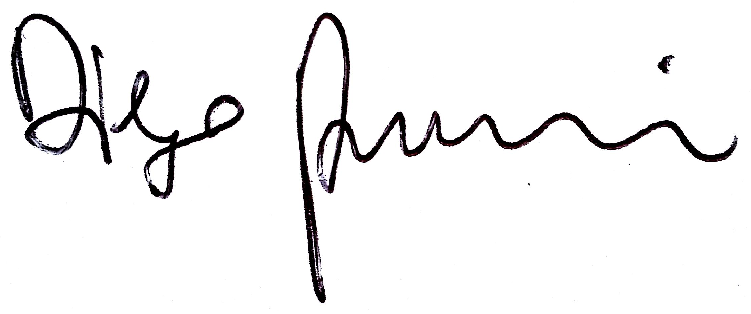
\includegraphics[width=5cm]{./firma_Diego.png}\\
%\end{center}
\end{flushleft}

Diego Bruciaferri \hspace{8cm} \today



\end{document}